\paragraph{Polarization signature of magnetized filaments}
The real space kernels give us a better intuitive understanding of the $E/B$ modes associated with physical objects.  For example, a simple model for a magnetize filament has the magnetic field threaded along a linear gas overdensity.  Precession of the dust grains around the magnetic field leads to a net polarization perpendicular to the magnetic field (and perpendicular to the filament overall).  For a filament aligned North--South, the polarization will be horizontal or $Q<0$, $U=0$ (left pane of \fig{fig:polfilaments}).  The Green's function kernels for horizontal polarization are rotated by 90 degrees relative to the components of $\cal{M}_G$ in \fig{fig:vis_kernel}.

The kernel can be thought of as the orientable nib of a calligraphy pen or paintbrush that we can trace along the filament.  The positive components for the $E$ part of the Green's function align and reinforce along the filament, and so the filament is highlighted as a segment with $E>0$.  Since the overdensity will also have emission in total intensity, this naturally predicts a positive $TE$ correlation for magnetized filaments.  The $E$ pattern is somewhat negative along the outside of the filament, also a consequence of the kernel shape.

The $B$ part of the Green's function, traced along the filament, cancels itself except at the filament ends.  This results in a non-zero $B$ pattern for the filament.  For a North--South filament, the $B$-mode pattern is positive on the North-East and South-West, and negative in the North-West and South-East.


The non-zero $B$ result is somewhat surprising given that the polarization pattern is symmetric to both horizontal and vertical reflections through the filament center.  However, unlike a complete ring, this filament is not a configuration with a definite parity.  Because the scalar polarization descriptions are coordinate independent, the $E/B$ patterns do not depend on the orientation of the filament.  A filament inclined at $45^\circ$ will have a similar $E/B$ pattern, but different reflection symmetries.  

%\revisit{A stacking analysis of Planck data \citep{2016A&A...586A.141P} sees $E>0$ along filaments (selected from intensity data), but no $B$-mode signal is above the noise.  We predict that it should be there in higher fidelity data.}
\revisit{A stacking analysis of Planck data \citep{2016A&A...586A.141P} sees $E>0$ along filaments (selected from intensity data), but claim no $B$-mode signal. We predict that a B-mode signal from filaments is present. A naive filament stacking analysis is only ideal for making E-mode detections. For detecting B-modes from filaments requires a more careful edge stacked filaments analysis. While its detectability from Planck requires more study, it should definitely be detectable in higher fidelity data.}

The intuition from the real-space kernels holds also when we distort the shape of the filament.  If the filament were bent around into a circle \comment{Not for an ellipse right? Maybe constant curvature argument is more general and more precise}, the positive and negative parts of the $B$ pattern will cancel, and we are left with a hoop of pure $E$ pattern.  The same general description holds for a spiral-shaped filament, which can can be viewed as distortion of the straight filament.  The filament is highlighted by positive $E>0$.  The $E$-pattern is more negative on the interior of a curve than on the exterior, and the concentric rings of filamentary structure make an increasingly negative $E$ value inside.  The $B$-pattern is again concentrated at the ends of the filament in an oriented pair of positive/negative fluctuations.
 
 
\begin{figure}
  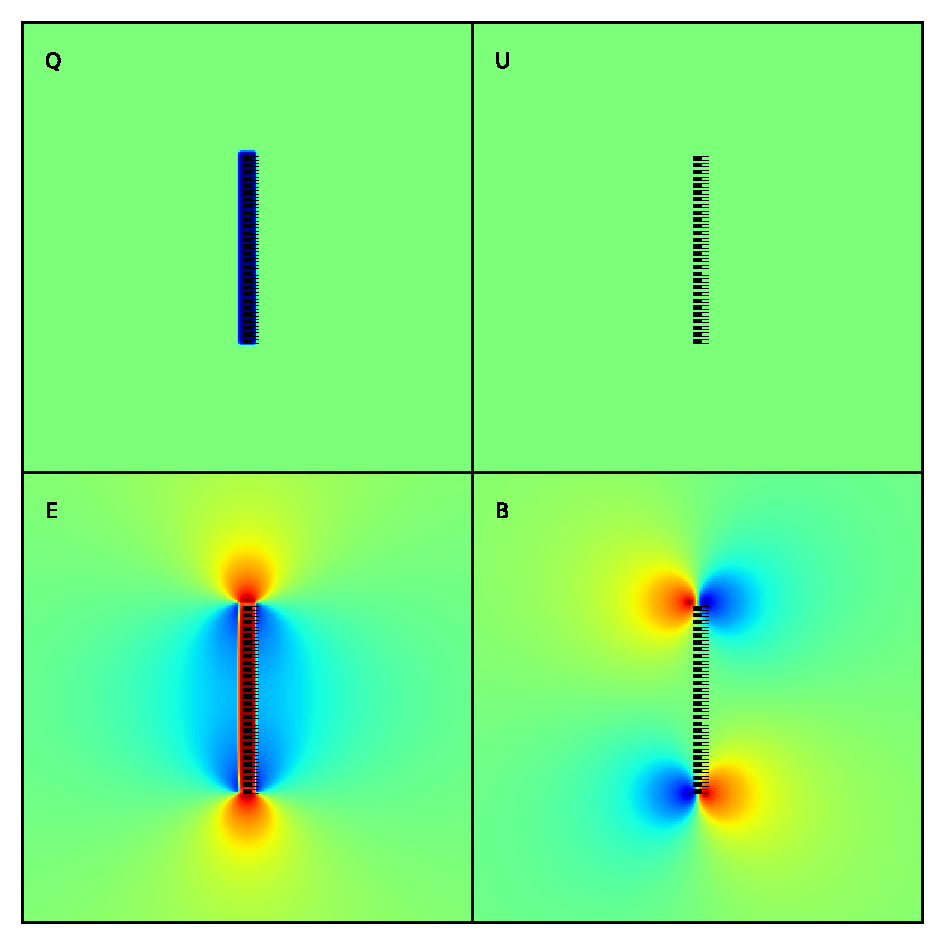
\includegraphics[width=0.5\columnwidth]{line.pdf}
  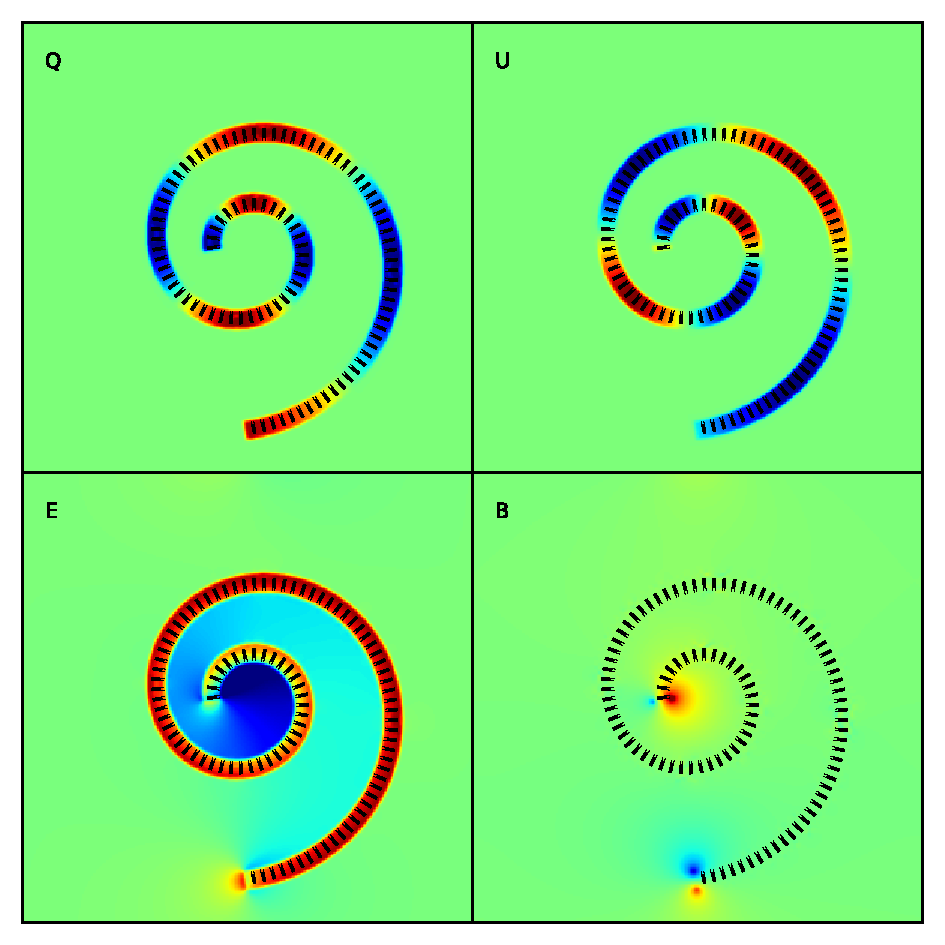
\includegraphics[width=0.5\columnwidth]{spiral.pdf}
  \caption{
    The polarization signals of toy filament structures.
    In a filament organized perfectly along a magnetic field line, the polarization will be perpendicular to the filament direction.  The $E/B$ modes of filaments are in some ways easier to think about than the Stokes parameters.
    Left panels: in a straight filament, the E-mode is positive along the filament and at the ends, but negative along the sides.  B-modes are only non-zero at the ends.  Right panels: in a curved filament, the E-mode is again positive along the filament.  Outside the filament, the $E$-mode is more negative on the interior of the curve than the exterior.  The $B$-modes are again non-zero only at the ends, and are akin to the straight filament case.
    In all images, the longitude angle increases to the left (East in sky convention).}
  \label{fig:polfilaments}
\end{figure}




 

